\documentclass[conference]{IEEEtran}
\usepackage{cite}
\usepackage{amsmath,amssymb,amsfonts}
\usepackage{graphicx}
\usepackage{textcomp}
\usepackage{xcolor}
\usepackage{booktabs}
\usepackage{microtype}
\graphicspath{{figures/}}
\usepackage[hidelinks]{hyperref}

\begin{document}

\title{Dominance Redefined: Visualizing Max Verstappen's 2023 Formula 1 Season}

\author{\IEEEauthorblockN{Varun Brahma}
\IEEEauthorblockA{Department of Computer Science\\
University of San Francisco\\
San Francisco, CA, USA\\
Email: vbrahma@dons.usfca.edu}
}

\maketitle

\begin{abstract}
Max Verstappen's 2023 Formula 1 season is often summarized through headline records --- 19 wins from 22 starts, 575 points --- but raw totals alone do not explain how the championship lead accumulated, how much of it can be attributed to the car, or how the season compares with other elite performances. This project presents an interactive visualization system that examines the season at four levels: race-by-race championship progression, comparison with teammate Sergio P\'erez, comparison with historically strong Formula 1 seasons, and comparison with peak athletes from other sports. The visualizations combine animated standings, small multiples, normalized parallel coordinates, and empirical cumulative distribution functions to move from raw race statistics toward more careful cross-era and cross-sport comparison. The system shows that Verstappen's separation from the field emerged through sustained mid-season expansion of his lead, exceeded his teammate's results by 290 points despite identical machinery, ranked among the strongest single seasons in Formula 1 history when measured by rate metrics rather than totals, and remained comparable with elite seasons in other sports when each performance was translated to a sport-relative percentile. The report also discusses the limits of normalization, the design choices behind each view, and the tradeoffs involved in comparing unlike competitive environments.
\end{abstract}

\begin{IEEEkeywords}
information visualization, sports analytics, Formula 1, D3.js, small multiples, parallel coordinates, empirical cumulative distribution function
\end{IEEEkeywords}

\section{Introduction}
Max Verstappen's 2023 Formula 1 season is remembered as dominant, but that description becomes more interesting when it can be measured. A final points total reveals only the endpoint of a season; a constructor advantage can obscure the driver's individual contribution; and raw records from different eras are difficult to compare when scoring systems and season lengths change. This project asks a more precise question: \emph{what does the 2023 season look like when it is examined over time, against the closest available control, across Formula 1 history, and against elite seasons in other sports?}

The system is designed for readers who understand basic computing concepts but are not visualization specialists. Rather than relying on one summary chart, it uses coordinated narrative sections that progressively widen the lens from the 2023 championship to historical and cross-sport comparison. The premise that each question demands a different form of fairness drives the choice of a different visual idiom for each section, following established principles of overview-before-detail, aligned comparison, and careful transformation of data before direct comparison \cite{munzner2014visualization,wilke2019fundamentals,segel2010narrative}. The resulting interactive site presents this analysis as a guided visual narrative \cite{brahma2026verstappen}.

The project objectives are:
\begin{itemize}
    \item Show how Verstappen's lead developed across the 22-race 2023 season.
    \item Separate driver performance from car performance by comparing Verstappen with teammate Sergio P\'erez in the same Red Bull RB19.
    \item Compare Verstappen's 2023 season with historically strong Formula 1 seasons using normalized rate metrics.
    \item Compare sustained relative performance across sports without treating unlike raw statistics as directly equivalent.
\end{itemize}

\begin{figure}[t!]
\centerline{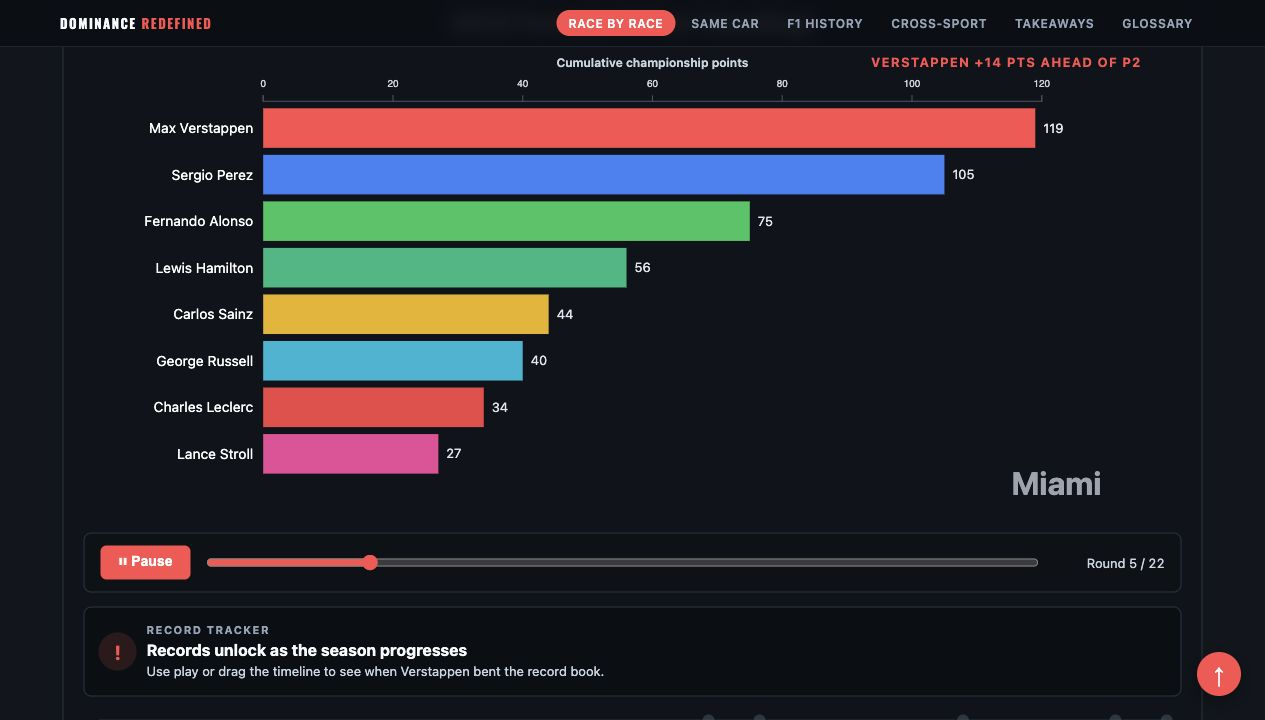
\includegraphics[width=\columnwidth]{championship.png}}
\caption{Objective 1: the bar-chart race shows cumulative standings at each round. In the frame captured here Verstappen already leads after Miami, while the slider and animation in the live system allow the reader to inspect how that advantage later becomes a decisive margin.}
\label{fig:race}
\end{figure}

\section{Related Work}
This project draws on three strands of prior work: general information-visualization principles, sports visualization, and prior Formula 1 analysis.

\emph{Information-visualization principles.} Munzner's task-centered framing motivates choosing a different chart for each analytical question instead of forcing one visual form to answer everything \cite{munzner2014visualization}. Wilke's discussion of small multiples shaped the teammate view, where aligned panels make differences legible without overplotting \cite{wilke2019fundamentals}. Segel and Heer's narrative-visualization framework is especially relevant because the final site is neither a static dashboard nor an author-controlled slideshow: it uses a guided sequence of sections while still allowing reader-driven exploration inside each view \cite{segel2010narrative}. Hullman and Diakopoulos's work on visualization rhetoric also informed the choice to surface limitations alongside results \cite{hullman2011visualization}, and Shneiderman's overview-zoom-details mantra underpins the within-section interaction patterns \cite{shneiderman1996eyes}.

\emph{Sports visualization.} Perin et al.\ argue that athletics data is particularly rich because it combines temporal, comparative, and narrative questions, making it a fertile setting for interactive analysis \cite{perin2018sports}. Their survey also highlights the recurring difficulty of comparing performances across rule changes, formats, and field sizes, which directly motivated the historical and cross-sport sections of this project.

\emph{Formula 1 analysis.} Van Kesteren and Bergkamp's Bayesian decomposition of driver skill and constructor advantage shows that the driver-vs.-car question is analytically important rather than a fan-level intuition, and supports the choice of teammate comparison as a practical control \cite{vankesteren2023f1}. Public-facing Formula 1 comparisons helped shape the historical-benchmarking direction of this project \cite{seymour2023f1,sportschord2023verstappen}. The implementation uses D3.js because it supports direct binding between data and document structure for bespoke interactive graphics \cite{bostock2011d3,murray2017interactive}.

\section{Approach}

\subsection{Data Preparation}
The project begins with race-level Formula 1 data for the 2023 season, primarily sourced from the publicly available JDAustralia Kaggle dataset \cite{jdaustralia2023f1}, and derives local CSV files for cumulative standings, teammate comparison, historical rate metrics, and cross-sport event outcomes.

\subsubsection{Why the parallel-coordinates plot must be normalized}
An early version of the historical comparison plotted seasons on \emph{raw counts}: wins, podiums, poles, fastest laps, points, and DNFs (Fig.~\ref{fig:pcp-raw}). That version was misleading for two compounding reasons. First, season length varies dramatically across eras --- Ascari 1952 ran a 6-race calendar, Senna 1988 ran 16, and Verstappen 2023 ran 22 --- so a driver with more starts can outscore a driver with a perfect rate. Second, the scoring system itself has changed: 1952 paid 9 points for a win, 1988 paid 9, and the modern system pays up to 26 (with sprint and fastest-lap bonuses). On a raw-count axis, Ascari's perfect 6-for-6 season collapses near the bottom while Verstappen's 22-race total dominates every axis, conflating ``season length and scoring inflation'' with ``driver quality.'' Converting each count into a per-race rate, and converting points into a fraction of the maximum points available that season, removes both confounds and lets the chart compare \emph{season profiles} rather than \emph{cumulative magnitudes}.

\begin{figure}[t!]
\centerline{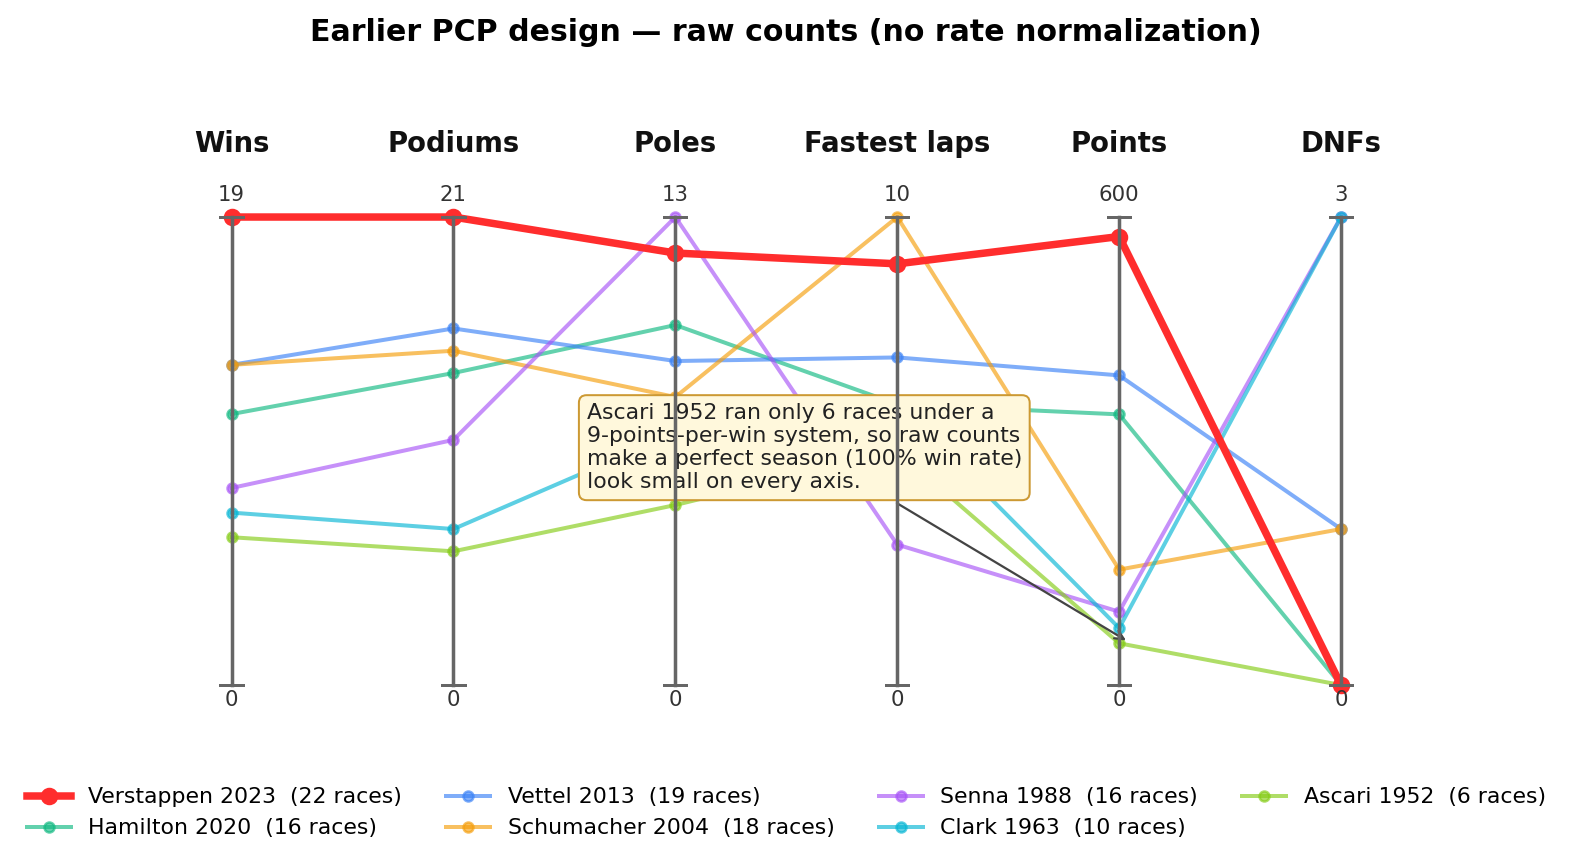
\includegraphics[width=\columnwidth]{pcp_raw.png}}
\caption{Earlier PCP design using raw counts. Verstappen 2023 dominates every axis, but the chart is misleading: Ascari 1952's perfect 6-for-6 season is squashed near the bottom of every axis because his calendar was shorter and his scoring system paid fewer points per win. This motivated the switch to per-race rates and points-capture fraction (Fig.~\ref{fig:history}).}
\label{fig:pcp-raw}
\end{figure}

The final parallel-coordinates plot therefore uses: win rate (wins divided by races), podium rate (podiums / races), pole rate (poles / races), fastest-lap rate (fastest laps / races), points capture (points scored divided by the maximum points available given the season's scoring system), and reliability (one minus the DNF rate). Each axis is a percentage or rate, so seasons of different lengths sit on a comparable scale.

For cross-sport comparison, every event result is translated into a sport-relative percentile based on the size of the competitive field at that event, so that a Formula 1 race in a 20-car field, a tennis tournament in a 128-player draw, and an Olympic swimming final among eight athletes can be plotted on a shared scale (Section~\ref{sec:methodology}).

\subsection{Visualization Design}
The final site contains four main views. First, an animated bar-chart race shows the evolving championship standings and makes the widening lead visible over time. Second, paired season totals and small multiples compare Verstappen with P\'erez, using the teammate as the closest practical control for machinery. Third, a parallel-coordinates chart compares historically strong Formula 1 seasons through normalized rate metrics. Fourth, an empirical cumulative distribution function (ECDF) plot compares sustained near-best performance across sports after translating each athlete's event results into percentiles.

\subsection{Cross-Sport Percentile Methodology}\label{sec:methodology}
The cross-sport view is the most analytically ambitious section of the system, so its transformation is described explicitly. For each athlete-season, the underlying records are event-level finishing ranks in that sport's natural unit: race finish position (Formula 1), tournament finish position (tennis), match-impact rank within a league season (soccer), innings-impact rank within a season (cricket), and Olympic-final finish position (swimming). For each event $i$ with finish rank $r_i$ in a field of size $N_i$, a sport-relative percentile is computed as $p_i = (N_i - r_i + 1) / N_i$, so that a win in any field produces $p_i = 1$ and weaker finishes produce smaller percentiles in proportion to the field size. The ECDF plot then summarizes the distribution of $\{p_i\}$ for each athlete-season; curves shifted toward the upper right indicate that the athlete spent a larger fraction of their events near the top of their own competitive field. This transformation avoids the misleading suggestion that a fifth-place finish means the same thing in fields of 8, 20, and 128 competitors. The model treats field size as the principal source of comparability and does not attempt to correct separately for tournament structure (single-elimination versus round-robin) or for differences in how impact is operationalized in team sports; those simplifications are revisited in the Limitations subsection.

\subsection{Iterations and Challenges}
The central design challenge was that each question demanded a different form of fairness. Raw totals were appropriate inside one season but misleading across eras; teammate comparison was more informative than constructor comparison for separating driver from car; and cross-sport rankings required transformation before any visual comparison could be defensible. Several weaker directions were corrected during ideation rather than after full implementation. The earliest proposal emphasized cumulative line charts, broad multi-driver comparison, and qualifying-versus-finishing analysis, but those ideas were narrowed once the project objectives became clearer. The revised plan replaced them with four more deliberate lenses: within-season progression, teammate comparison, historical Formula 1 benchmarking, and cross-sport context. By the alpha release, the small-multiples teammate comparison and bar-chart race were already established as the analytical backbone, while the later historical and ECDF views were still being developed. Most subsequent changes were stylistic and usability-focused: layout, hierarchy, annotations, color consistency, navigation, and interaction polish rather than changes to the underlying analytical structure.

The most substantive late refinement deserves a paragraph of its own. An earlier version of the cross-sport ECDF used \emph{raw finishing ranks} as the x-axis (Fig.~\ref{fig:older-ecdf}), so that a rank of, say, 5 was plotted at the same x-position regardless of whether the field was 8, 20, or 128 competitors. That version was visually readable but quietly inflated equivalence between fundamentally different field sizes. Replacing the rank axis with the sport-relative percentile defined in Section~\ref{sec:methodology} produced a more defensible comparison and made the discarded design itself a useful illustration of why the transformation matters.

\begin{figure}[htbp]
\centerline{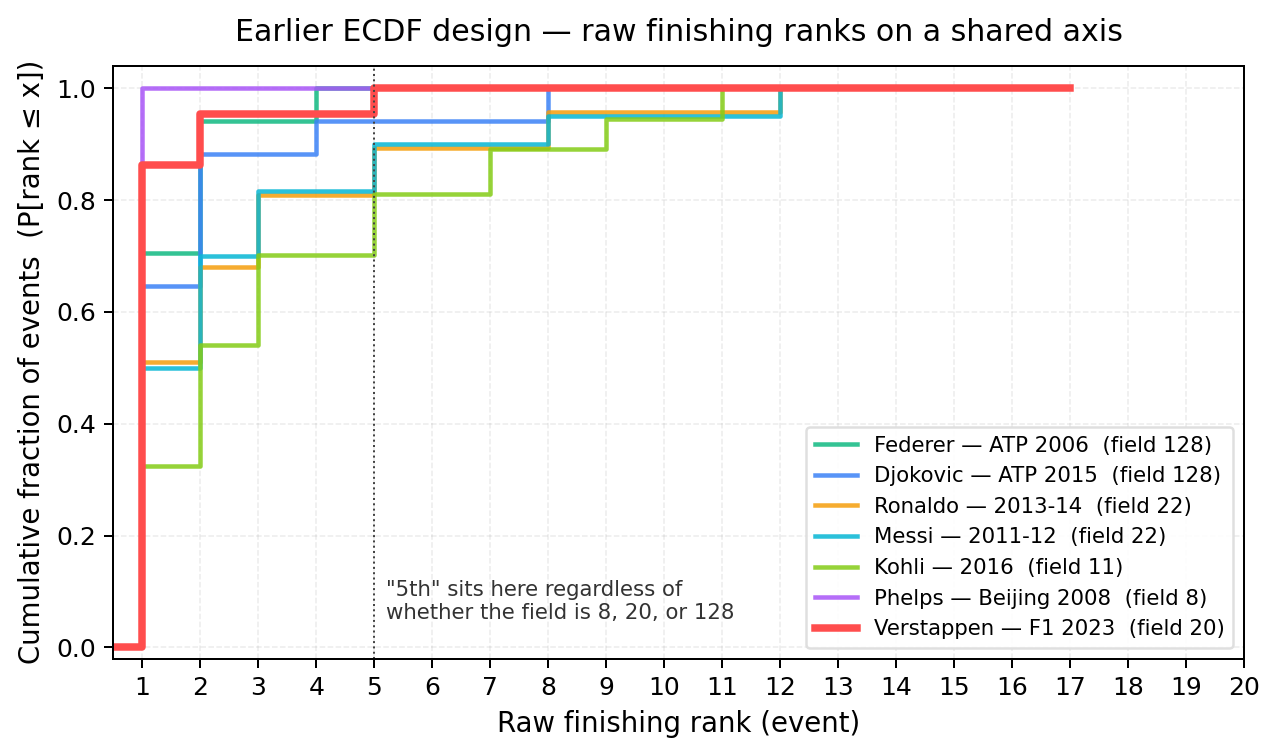
\includegraphics[width=\columnwidth]{old.png}}
\caption{Reconstruction of the earlier ECDF design that plotted raw finishing ranks across sports on a shared x-axis. The chart is visually readable but quietly implies stronger comparability than the data supports: a finish of fifth means very different things in fields of 8, 20, and 128 competitors. This is the limitation that motivated the final percentile-based redesign described in Section~\ref{sec:methodology}.}
\label{fig:older-ecdf}
\end{figure}

\section{Results}

\subsection{Objective 1: Within-Season Progression}
The animated standings view shows that Verstappen's lead was not merely present at the final race; it accumulated through sustained mid-season expansion. After the opening round in Bahrain, Verstappen led P\'erez by only 7 points, and the gap remained within 15 points through the first four races. The margin reached 39 points after Monaco (round 6) and crossed 100 points after the British Grand Prix (round 10). By the Italian Grand Prix (round 14) the gap was 145 points, and the championship was mathematically clinched at Qatar (round 17) with five races still to run. Figure~\ref{fig:race} captures an early-to-middle-season frame in which Verstappen leads but has not yet produced the final-season chasm, making the later expansion meaningful rather than inevitable.

\subsection{Objective 2: Driver Versus Car}
The teammate comparison shows that identical machinery did not produce identical outcomes. In the same Red Bull RB19, Verstappen recorded 575 points to P\'erez's 285, 19 wins to 2, and 21 podiums to 9. The 290-point intra-team gap was larger than the gap separating P\'erez from third place in the drivers' championship that year, which is the strongest practical evidence available in the dataset that the RB19 was a major enabling factor but not a complete explanation of the final margin (Fig.~\ref{fig:teammate}).

\subsection{Objective 3: Formula 1 History}
The normalized historical view positions 2023 among the strongest single Formula 1 seasons ever while preserving nuance. Across the seasons compared --- Ascari 1952, Clark 1963, Senna 1988, Schumacher 2004, Vettel 2013, Hamilton 2020, and Verstappen 2023 --- Verstappen leads on absolute totals and ranks at or near the top on win rate (19/22, 86.4\%) and podium rate (21/22, 95.5\%). The chart deliberately preserves cases where his season is exceeded: Ascari 1952 posted a perfect 100\% win rate over a 6-race calendar, and Senna 1988 reached a higher pole rate (13 poles in 16 races, 81.3\%) than Verstappen's pole rate in 2023. Surfacing these counterexamples is the analytical point of the chart: it prevents the visualization from collapsing history into a single unqualified ranking (Fig.~\ref{fig:history}).

\subsection{Objective 4: Cross-Sport Comparison}
The ECDF view makes cross-sport comparison possible without pretending that a race finish, a tennis tournament result, and a swimming final are the same measurement. After each event is translated to a sport-relative percentile (Section~\ref{sec:methodology}), Phelps's Beijing 2008 curve sits at the upper bound, reflecting eight first-place finishes in fields of eight. Verstappen's curve clusters near the top of his own competitive field, with the visible deviation corresponding to his fifth-place finish at Singapore in a 20-car field. Federer 2006 and Djokovic 2015 spend most of their tournaments at or near the win, with longer lower tails that reflect the deeper 128-player draws of the ATP Tour (Fig.~\ref{fig:ecdf}). The view supports a comparison of sustained relative excellence rather than a claim that the sports themselves are directly interchangeable.

\begin{figure}[htbp]
\centerline{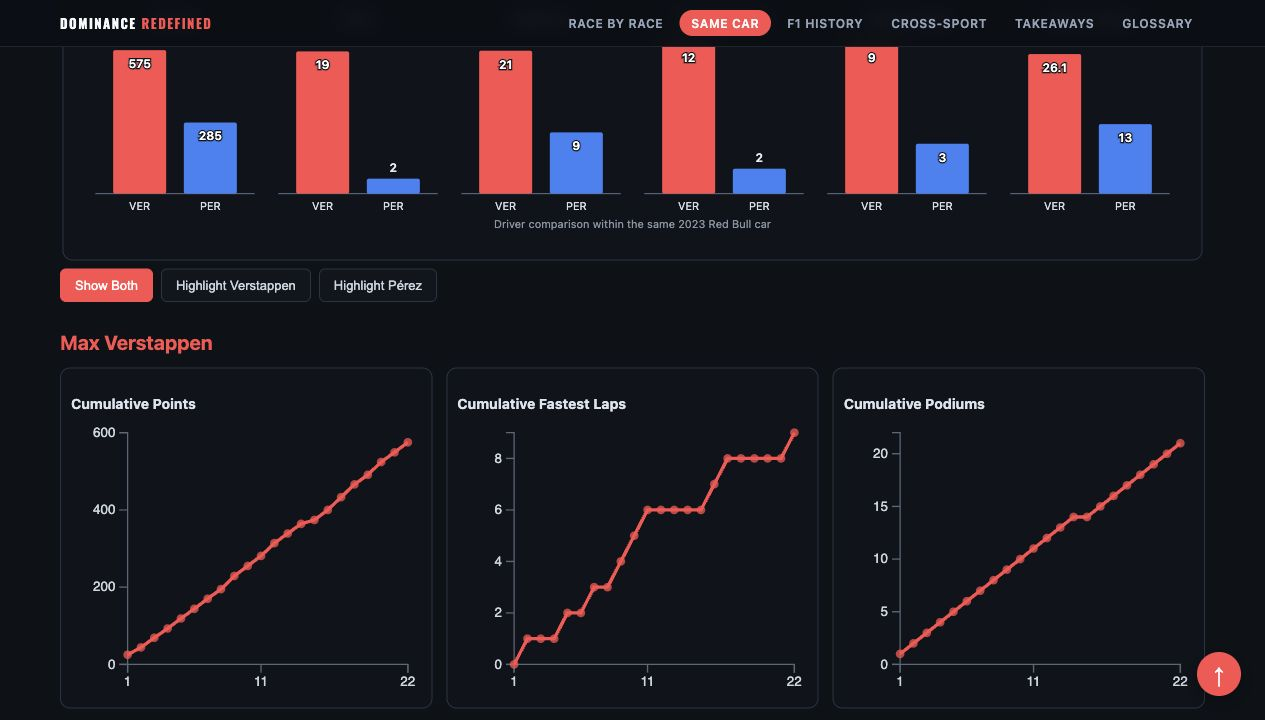
\includegraphics[width=\columnwidth]{SmallMultiples.png}}
\caption{Objective 2: season totals and the first row of small multiples compare Verstappen with P\'erez in the same RB19. The paired bars make the 290-point overall gap immediate, while the aligned time series show that the difference accumulates throughout the season rather than emerging from a single round.}
\label{fig:teammate}
\end{figure}

\begin{figure}[htbp]
\centerline{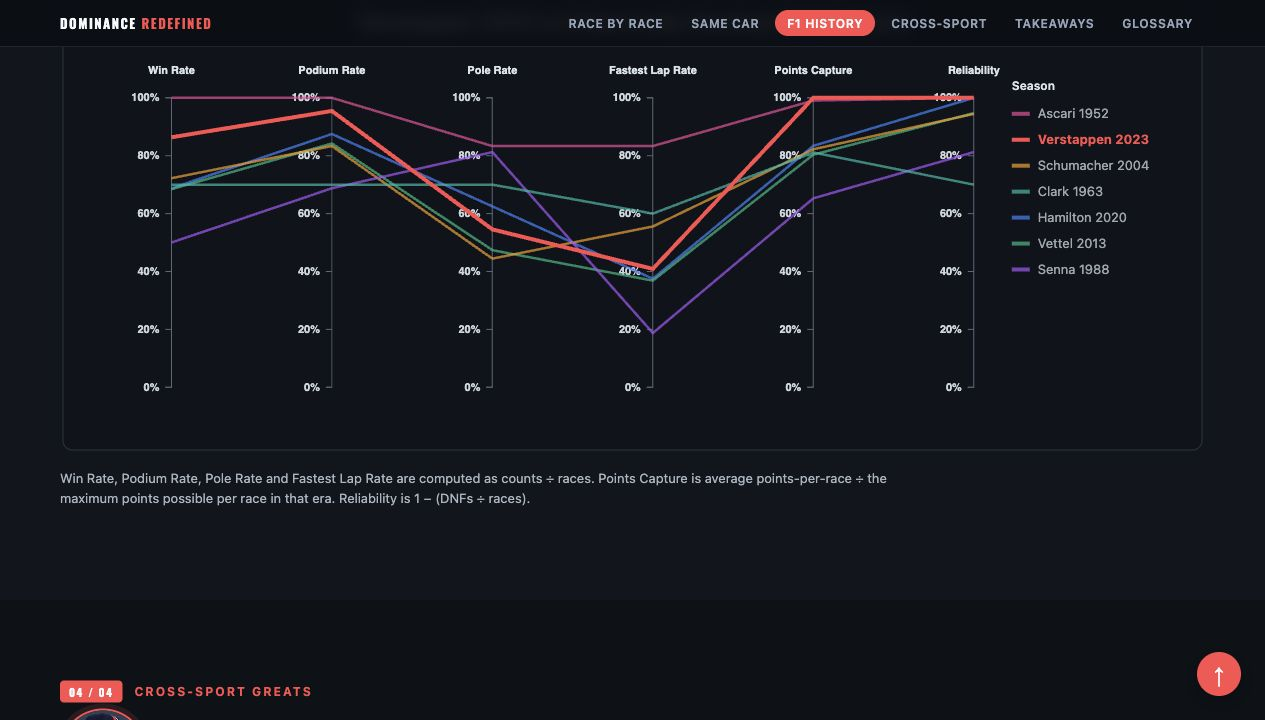
\includegraphics[width=\columnwidth]{PCP.png}}
\caption{Objective 3: normalized parallel coordinates compare historically strong Formula 1 seasons across rate metrics. The chart preserves nuance: Verstappen 2023 leads on most axes, while Ascari 1952 still reaches 100\% on win rate and Senna 1988 exceeds him on pole rate.}
\label{fig:history}
\end{figure}

\begin{figure}[htbp]
\centerline{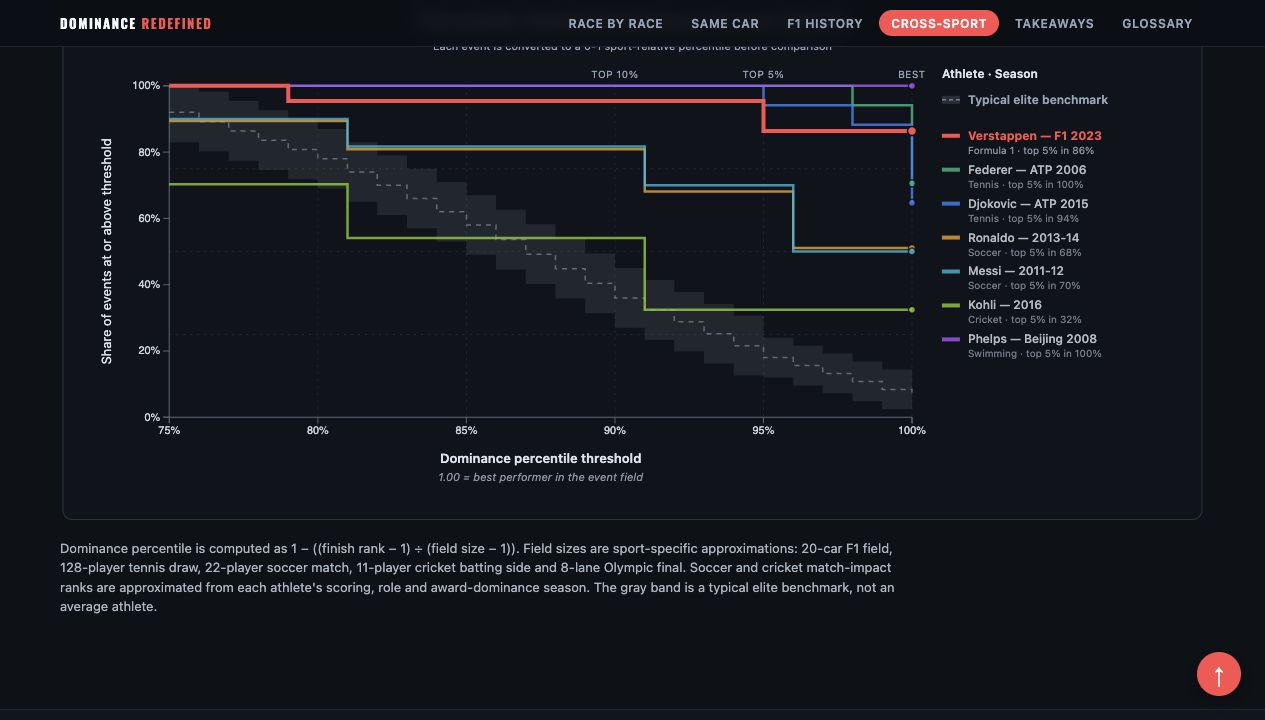
\includegraphics[width=\columnwidth]{ECDF.png}}
\caption{Objective 4: the ECDF view compares sustained relative performance after each event is translated to a sport-relative percentile (Section~\ref{sec:methodology}). Curves shifted toward the upper right indicate that the athlete spent a larger fraction of events near the top of their own competitive field.}
\label{fig:ecdf}
\end{figure}

\subsection{Measuring Success}
Success was measured by whether each visualization answered a distinct project objective, whether viewers could recover the intended comparison without relying on prose alone, whether interactive controls exposed additional detail without hiding the main claim, and whether the system became more conservative in its claims as the analytical scope widened beyond Formula 1. The final design is successful when it communicates not simply that Verstappen was dominant, but \emph{how}, \emph{relative to whom}, and \emph{under what assumptions}.

\section{Discussion}
The overall approach is promising because it avoids forcing one chart to answer every question. The strongest design decision is the progressive widening of context: the reader first sees a familiar season story, then a controlled teammate comparison, then a historical comparison, and only afterward a cautious cross-sport abstraction. This order earns the more ambitious claims rather than presenting them as spectacle.

\subsection{Limitations}
Several limitations are explicit. First, the analysis covers a single season for the driver and therefore cannot speak to the consistency of his form over a career. Second, the historical normalization assumes that scoring-system effects are approximately linear after rate conversion, which is reasonable but not airtight. Third, the cross-sport percentile model treats field size as the principal source of comparability, but tournament structures differ in elimination dynamics: a 128-player single-elimination draw is not strictly equivalent to a round-robin league season even when both are translated to percentiles. Fourth, the soccer and cricket event ranks rely on impact-based approximations rather than naturally shared tournament structures, which is signalled in the captions but cannot be fully removed without different source data. Fifth, the system has not been evaluated through a formal user study, so claims about reader comprehension are based on design reasoning rather than empirical measurement.

\subsection{Lessons}
The project reinforced that fairness in visualization is not one fixed rule; it depends on the question being asked and the transformations needed to make comparison meaningful. If starting again, I would formalize the data model earlier and decide the cross-sport comparison rule sooner. The project became stronger once the design stopped asking, ``what else can be shown?'' and started asking, ``what comparison is defensible here?''

\section{Future Work}
Future work could add linked highlighting across views, user-controlled metric weighting for the historical comparison, richer annotation of rule changes across Formula 1 eras, and a more rigorous cross-sport dataset built from event-level records rather than hand-curated approximations. A lightweight user study could test whether readers correctly distinguish raw totals, normalized rates, and percentile-based dominance. Sensitivity analysis of the percentile model --- for example, varying the field-size assumption or replacing the linear percentile with a position-weighted scoring rule --- would also strengthen the cross-sport section.

\section{AI Use Disclosure}
Generative AI was used as a support tool during the project for wording refinement, limited CSV cleanup and name normalization, and finding possible resources for manual review. It was not treated as an authoritative data source: numeric values used in the final visualizations were checked against the underlying records before inclusion.

\section{Conclusion}
This project uses interactive visualization to turn a familiar sports claim into a sequence of testable comparisons. By moving from season progression to teammate control, historical normalization, and cross-sport percentiles, it shows that Verstappen's 2023 season was not merely record-setting but structurally separated from the field across multiple analytical frames. At the same time, the project argues that good visualization should sharpen claims rather than inflate them: the strongest contribution of the system is not the assertion that Verstappen was dominant, but the more careful framework that makes that assertion measurable and contestable.

\bibliographystyle{IEEEtran}
\bibliography{references}

\end{document}
